%Mohr 2018 round 1 - p17
%geo 2
Á myndinni sést ferhyrningurinn $ABCD$ þar sem nokkrar lengdir eru gefnar. Hver er lengd striksins $AB$?
\begin{center}
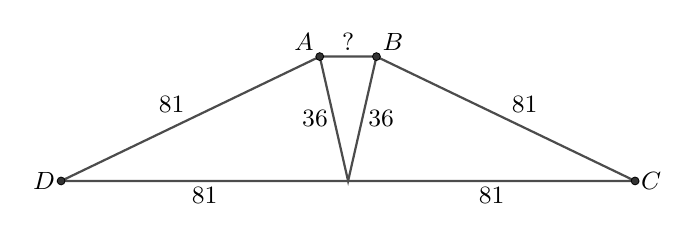
\begin{tikzpicture}[scale=0.045,
    dot/.style={circle, fill=black!80, draw=black, line width=0.3pt, inner sep=1pt},
    lbl/.style={font=\small, inner sep=2pt}]
  % --- data: |DM|=|MC|=|AD|=|BC|=81, |AM|=|BM|=36 ---
  % A=(x,y) with |A-M|=36, |A-D|=81  =>  x=-8, y=sqrt(36^2-8^2)
  \pgfmathsetmacro{\h}{sqrt(36^2-8^2)}

  \coordinate (D) at (-81,0);
  \coordinate (M) at (0,0);
  \coordinate (C) at (81,0);
  \coordinate (A) at (-8,\h);
  \coordinate (B) at (8,\h);

  % --- drawing ---
  \draw[black!70, thick] (D) -- (C) -- (B) -- (A) -- cycle;
  \draw[black!70, thick] (A) -- (M) -- (B);

  \path (D) -- (A) node[lbl, midway, above left] {$81$};
  \path (B) -- (C) node[lbl, midway, above right] {$81$};
  \path (D) -- (M) node[lbl, midway, below] {$81$};
  \path (M) -- (C) node[lbl, midway, below] {$81$};
  \path (A) -- (M) node[lbl, midway, left] {$36$};
  \path (B) -- (M) node[lbl, midway, right] {$36$};
  \path (A) -- (B) node[lbl, midway, above] {$?$};

  \node[dot] at (A) {}; \node[lbl, above left]  at (A) {$A$};
  \node[dot] at (B) {}; \node[lbl, above right] at (B) {$B$};
  \node[dot] at (C) {}; \node[lbl, right] at (C) {$C$};
  \node[dot] at (D) {}; \node[lbl, left]  at (D) {$D$};
\end{tikzpicture}
\end{center}
